%-*- coding: UTF-8 -*-
% notes.tex
%
\documentclass[UTF8]{article}
\usepackage{geometry}
\geometry{a4paper, centering, scale=0.8}
\usepackage{minted}
\usepackage{hyperref}
\usepackage{indentfirst}    % to indent the first paragraph of a section
\usepackage{graphicx}       % to insert figures
\usepackage{amsmath}        % to type some math equations
\usepackage{amssymb}        % to use some special math font
\usepackage{IEEEtrantools}  % to use IEEEeqnarray
\usepackage{ulem}           % to use stikeout command \sout{}
\usepackage{algorithm2e}    % to use algorithm environment

% Math notation
% refered to https://github.com/exacity/deeplearningbook-chinese/blob/master/math_symbol.tex
\newcommand{\Scalar}[1]{\mathit{#1}}                % Scalar, the default math font
\newcommand{\Vector}[1]{\boldsymbol{\mathit{#1}}}   % Vector
\newcommand{\Matrix}[1]{\boldsymbol{\mathit{#1}}}   % Matrix
\newcommand{\Tensor}[1]{\textsf{\textbf{#1}}}       % Tensor
\newcommand{\Set}[1]{\mathbb{#1}}                   % Set
\newcommand{\Cal}[1]{\mathcal{#1}}                  % Math Cal


\title{Deep Learning Specialization \\
        Neural Networks and Deep Learning \\
        Learning Notes}
\author{Du Ang \\ \texttt{du2ang233@gmail.com} }
\date{\today}

\begin{document}
\maketitle

\tableofcontents
\newpage

\section{Welcome}
\begin{quote}
    \emph{AI is the new Electricity. --- Andrew Ng}
\end{quote}

Electricity had once transformed countless industries: transportation, manufacturing, healthcare,
communications, and more.

AI will now bring about an equally big transformation.

\paragraph{Courses in this sequence (Specialization):}
\begin{enumerate}
    \item \emph{Neural Networks and Deep Learning}
    \item \emph{Improving Deep Neural Networks: Hyperparameter tuning, Regularization and
    Optimization}
    \item \emph{Structuring Machine Learning Projects}
    \item \emph{Convolutional Neural Networks}
    \item \emph{Sequence Models}
\end{enumerate}

\section{Introduction to Deep Learning}
\subsection{What is a neural network?}
It is powerful learning algorithm inspired by how the brain works.
\subsubsection{Single neural network}
Given data about the size of houses on the real estate market and you want to fit a function that
will predict their price. It is a linear regression problem because the price as a function of size
is a continuous output.

We know the prices can never be negative so we are creating a function called Rectified Linear Unit
(ReLU) which starts at zero.
\begin{figure}[ht]
    \centering
    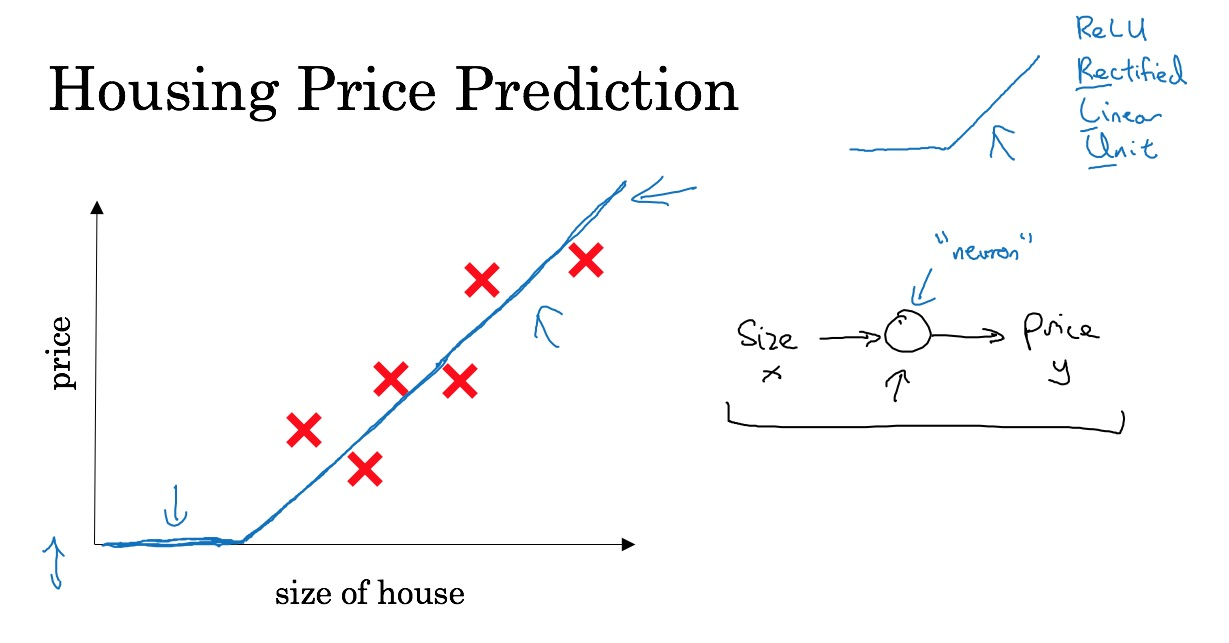
\includegraphics[width=40em]{figures/1-single-nn}
    \caption{The ``Housing Price Prediction'' problem. The input is the size of the house
    ($x$); The output is the price ($y$); The ``neuron'' implements the function
    ReLU.}
\end{figure}

\subsubsection{Multiple neural network}
The price of a house can be affected by other features such as size, number of bedrooms, zip code
and wealth. The role of the neural network is to predicted the price and it will automatically
generate the hidden units. We only need to give the inputs x and the output y.
\begin{figure}[ht]
    \centering
    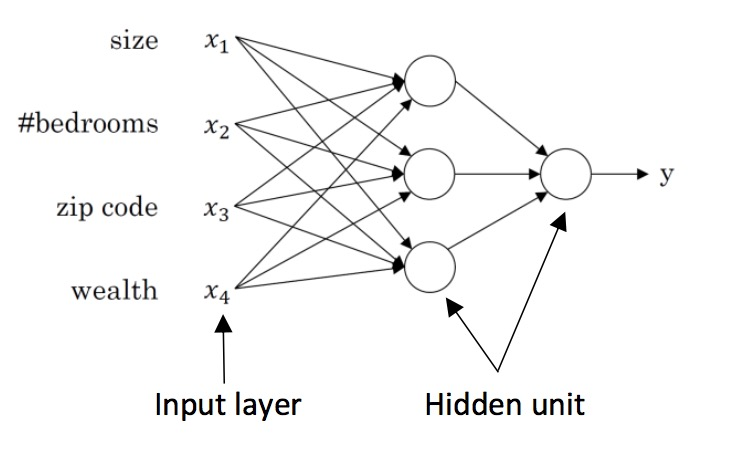
\includegraphics[width=40em]{figures/1-multiple-nn}
    \caption{Multiple neural network}
\end{figure}

\subsection{Supervised Learning}
In supervised learning, we are given a data set and already know about what our correct output
should look like, having the idea that there is a relationship between the input and the output.

Supervised learning problems are categorized into ``regression'' and ``classification'' problems.
In a regression problem, we are trying to predict results with a continuous output, meaning that we
are trying to map input variables to some continuous function. In a classification problem, we are
instead trying to predict results in a discrete output. In other words, we are trying to map input
variables into discrete categories.

Here are some example of supervised learning:
\begin{table}[ht]
\centering
\caption{Supervised Learning Applications}
\begin{tabular}{lllc}
\textbf{Input($x$)} & \textbf{Output($y$)} & \textbf{Application}
& \textbf{NN Types} \\ \hline
Home features & Price & Real Estate & Standard NN \\
Ad, user info & Click on ad? (0/1) & Online Advertising & Standard NN \\
Image & Object (1, ..., 1000) & Photo tagging & CNN \\
Audio & Text transcript & Speech Recognition & RNN \\
English & Chinese & Machine translation & RNN \\
Image, Radar info & Position of other cars & Autonomous driving & Custom/Hybrid \\
\end{tabular}
\end{table}

There are different types of neural network, for example, Convolutional Neural Network (CNN) used
often for image application and Recurrent Neural Network (RNN) used for one-dimensional sequence
data such as translating English to Chinese or a temporal component such as text transcript. As for
the autonomous driving, it is a hybrid neural network architecture.

\subsubsection{Structured vs unstructed data}
Structed data refers to things that has a defined meaning such as price, age whereas unstructed
data refers to thing like pixel, raw audio, text.

\subsection{Why is Deep Learning taking off?}
Deep learning is taking off due to a large amount of data available through the digitization of the
society, faster computation and innovation in the development of neural network algorithm.
\begin{figure}[ht]
    \centering
    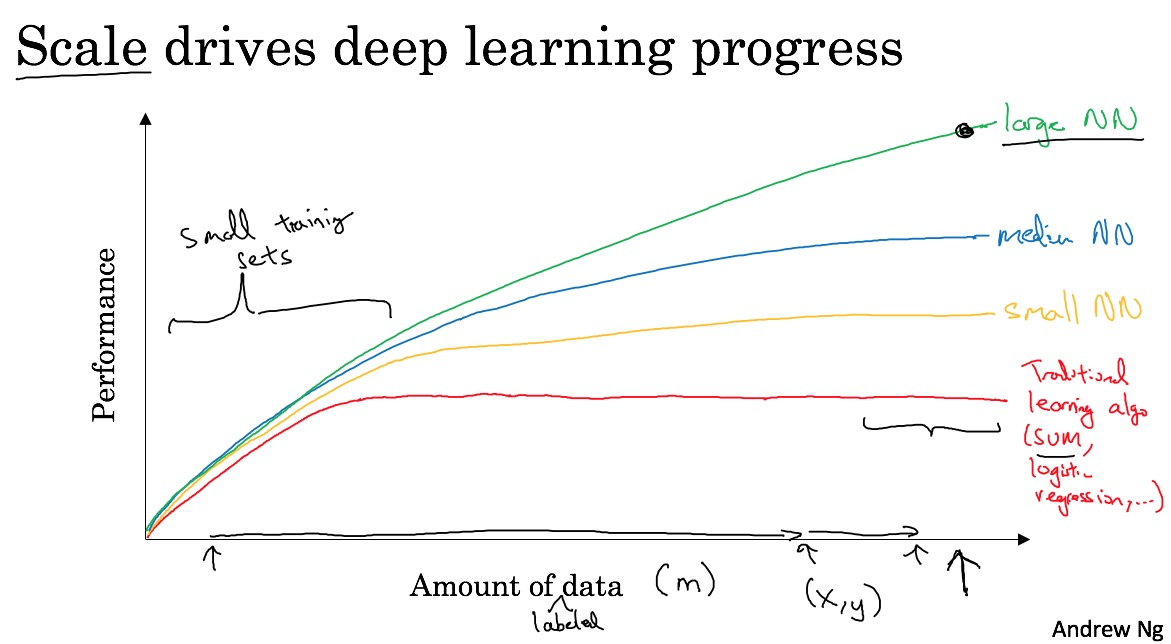
\includegraphics[width=40em]{figures/1-deep-nn-scale}
    \caption{Scale drives deep learning progress}
\end{figure}

Two things have to be considered to get to the high level of performance:
\begin{enumerate}
    \item Being able to train a big enough neural network
    \item Huge amount of labelled data
\end{enumerate}

The process of training a neural network is iterative:
\begin{figure}[ht]
    \centering
    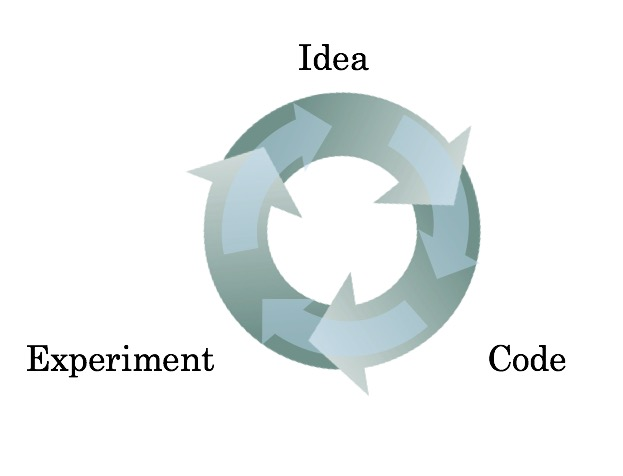
\includegraphics[width=25em]{figures/1-train-nn-process}
\end{figure}

It could take a good amount of time to train a neural network, which affects your productivity.
Faster computation helps to iterate and improve new algorithm.

\section{Neural Network Basics}
\subsection{Logistic Regression as a Neural Network}
\subsubsection{Binary Classification}
In a binary classification problem, the result is a discrete value output. For example:
\begin{itemize}
    \item account hacked (1) or compromised (0)
    \item a tumor malign (1) or benign (0)
\end{itemize}

\paragraph{Example: Cat vs Non-Cat}
The goal is to train a classifier that the input is an image represented by a feature vector,
$x$, and predicts whether the corresponding label $y$ is 1 or 0. In this case,
whether this is a cat image (1) or a non-cat image (0).

\begin{figure}[ht]
    \centering
    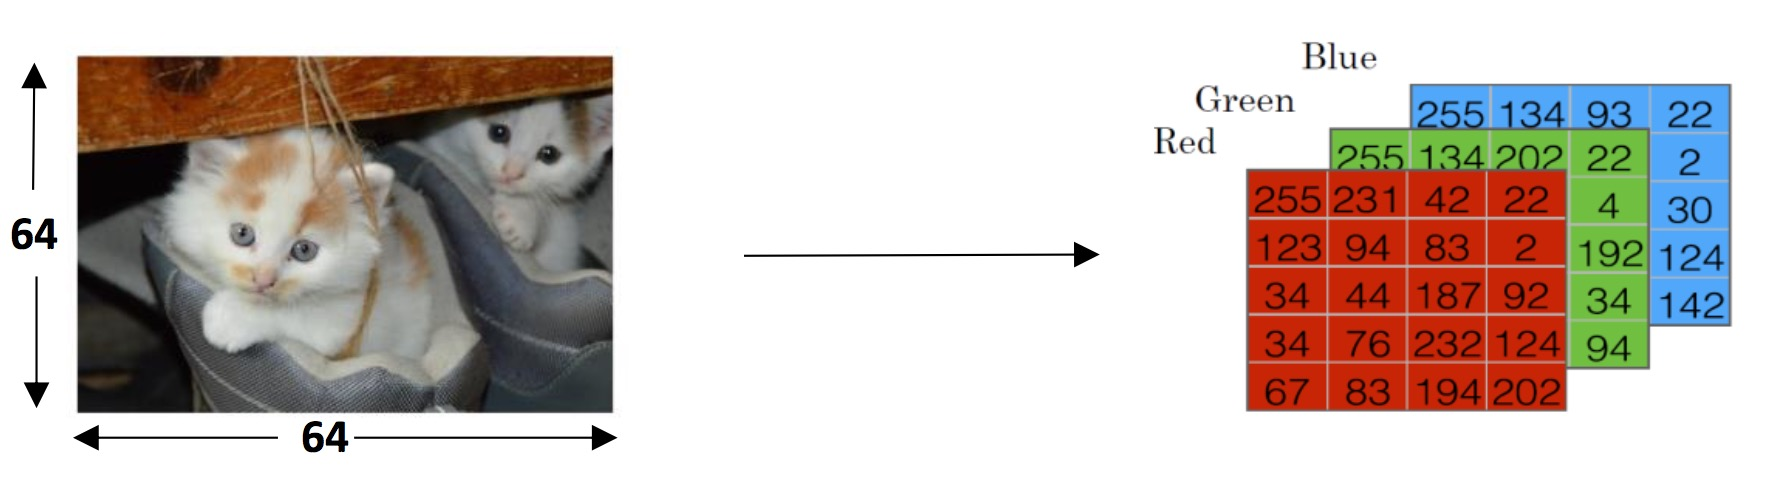
\includegraphics[width=35em]{figures/1-cat}
\end{figure}
An image is store in the computer in three separate matrices corresponding to the Red, Green, and
Blue color channels of the image. The three matrices have the same size as the image, for example,
the resolution of the cat image is 64 pixels $\times$ 64 pixels, the three matrices (RGB) are 64
$\times$ 64 each.

The value in a cell represents the pixel intensity which will be used to create a feature vector of
n-dimension. In pattern recognition and machine learning, a feature vector represents an object, in
this case, a cat or no cat.

To create a feature vector, $\Vector{x}$, the pixel intensity values will be ``unroll'' or
``reshape'' for each color. The dimension of the input feature vector $\Vector{x}$, is
$n_x = 64 \times 64 \times 3 = 12288$.
\begin{figure}[ht]
    \centering
    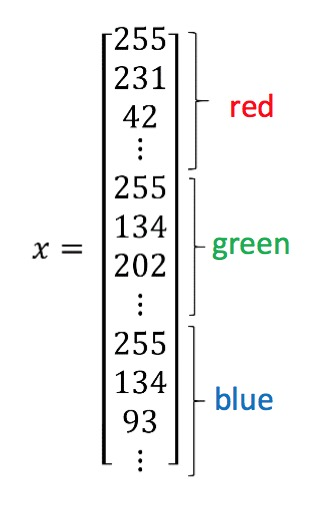
\includegraphics[width=10em]{figures/1-unrolled-image}
\end{figure}

\subsubsection{Notation}
single example: $(x, y)$, $x \in \Set{R}^{n_x}$, $y \in \{0, 1\}$

$m$ training examples: $\{(x^{(1)}, y^{(2)}), (x^{(2)}, y^{(2)}), ..., (x^{(m)}, y^{(m)})\}$

$m = m_{train}$ \qquad $m_{test}$ = the number of test examples

\begin{IEEEeqnarray*}{rCl}
    \Matrix{X} = \left[
        \begin{array}{cccc}
            \big| & \big| & & \big| \\
            \big| & \big| & & \big| \\
            \Vector{x}^{(1)} & \Vector{x}^{(2)} & \ldots & \Vector{x}^{(m)} \\
            \big| & \big| & & \big| \\
            \big| & \big| & & \big|
        \end{array}
    \right]
    \qquad
    \Matrix{X} \in \Set{R}^{{n_x} \times m}
\end{IEEEeqnarray*}

\begin{IEEEeqnarray*}{rCl}
    \Matrix{Y} = \left[
        \begin{array}{cccc}
            y^{(1)} & y^{(2)} & \ldots & y^{(m)}
        \end{array}
    \right]
    \qquad
    \Matrix{Y} \in \Set{R}^{1 \times m}
\end{IEEEeqnarray*}

In Python/NumPy, \mintinline{numpy}{X.shape = (n_x, m), Y.shape = (1, m)}.

\subsubsection{Logistic Regression}
Logistic regression is a learning algorithm used in a supervised learning problem when the output
$y$ are all either zero or one. The goal of logistic regression is to minimize the error between
its predictions and training data.

\paragraph{Example: Cat vs Non-Cat}
Given an image represented by a feature vector $x$, the algorithm will evaluate the probabilty of a
cat being in that image.

Given $x$, want $\hat{y} = P(y=1|x)$, $x \in \Set{R}^{n_x}$, $0 \leq \hat{y} \leq 1$

Parameters: $w \in \Set{R}^{n_x}$, $b \in \Set{R}$

Output: \sout{$\hat{y} = w^T x + b$} \quad $\hat{y} = \sigma (w^T + b)$, where
$\sigma(z) = \frac{1}{1+e^{-z}}$.
\begin{figure}[ht]
    \centering
    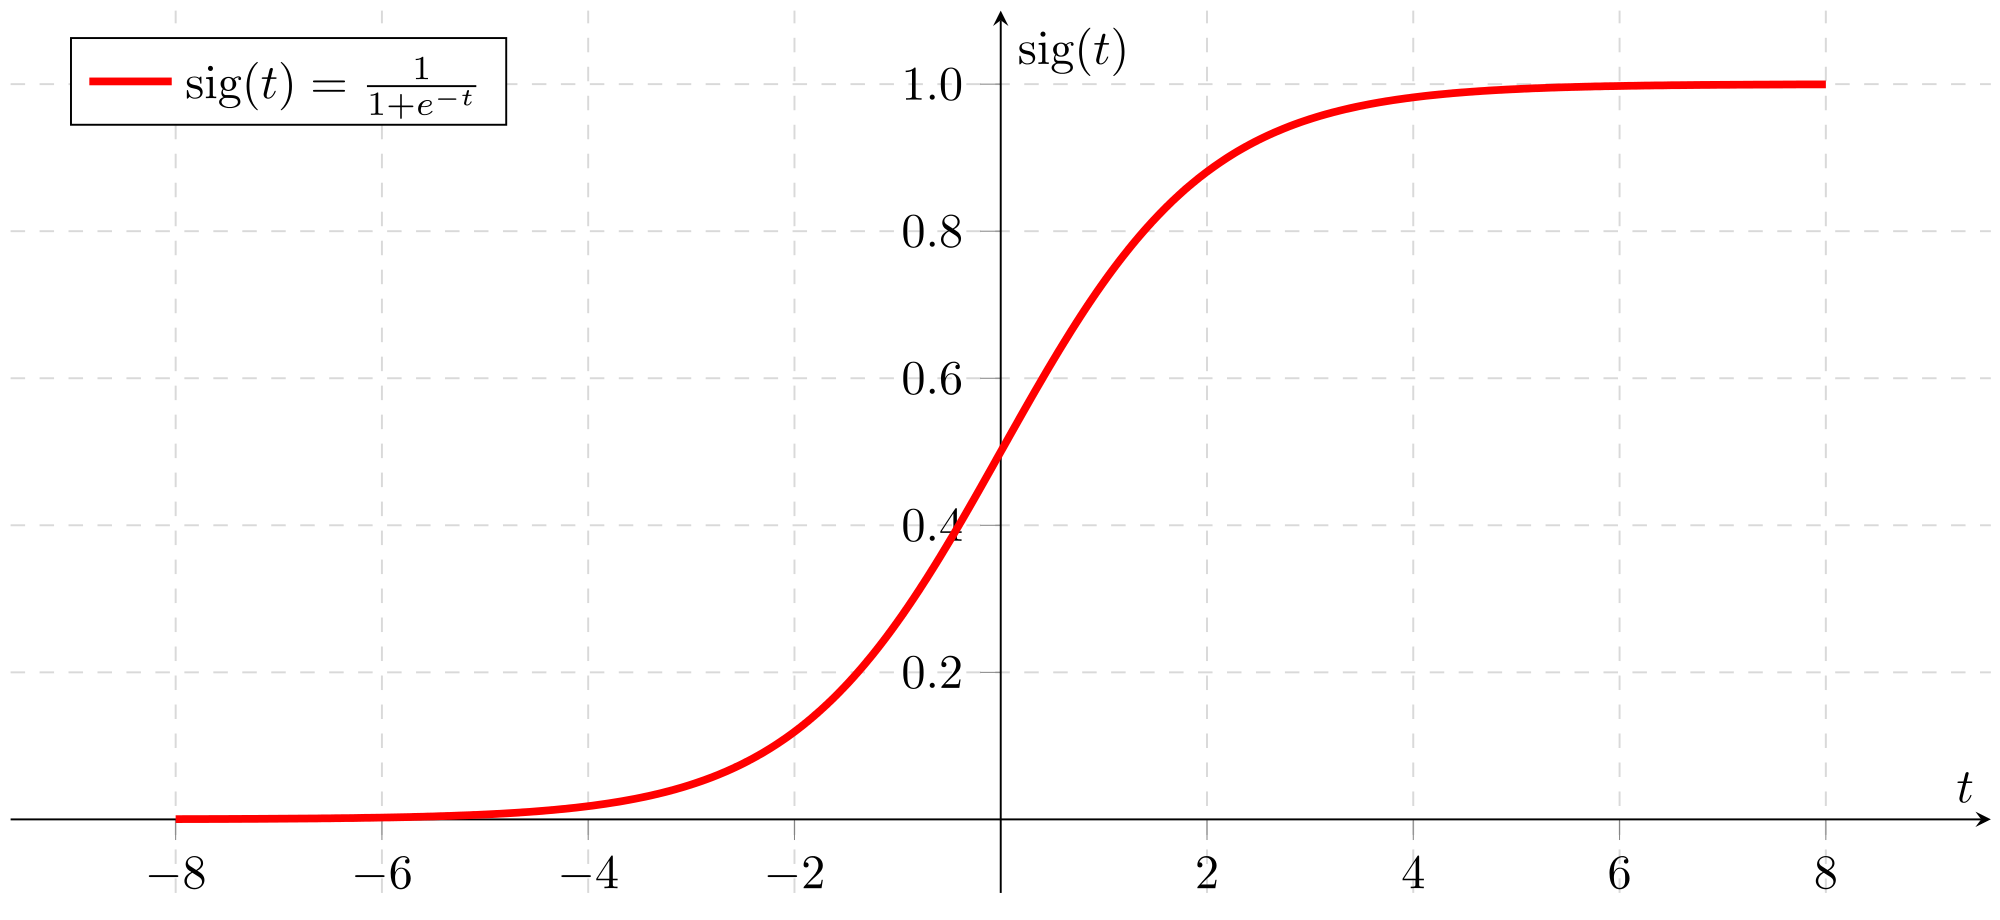
\includegraphics[width=25em]{figures/1-sigmoid}
    \caption{Sigmoid}
\end{figure}

$(w^T + b)$ is a linear function $(ax + b)$, but since we are looking for a probability constraint
between [0, 1], the sigmoid function is used. The function is bounded between [0, 1] as shown in
the graph above.

Some observations from the sigmoid function graph:
\begin{itemize}
    \item If $z$ is a large positive number, then $\sigma(z) = 1$
    \item If $z$ is small or large negative number, then $\sigma(z) = 0$
    \item If $z = 0$, then $\sigma(z) = 0.5$
\end{itemize}

\paragraph{Logistic Regression cost function}
$\hat{y}^{(i)} = \sigma (w^T x^{(i)} + b)$, where $\sigma(z^{(i)}) = \frac{1}{1+e^{-z^{(i)}}}$

Given $\{(x^{(1)}, y^{(2)}), (x^{(2)}, y^{(2)}), ..., (x^{(m)}, y^{(m)})\}$, want
$\hat{y}^{(i)} \approx y^{(i)}$.

\paragraph{Loss (error) function:} (for single example)
\begin{IEEEeqnarray*}{rCl}
    \Cal{L}(\hat{y}, y) = -(y\log{\hat{y}} + (1-y)\log(1-\hat{y}))
\end{IEEEeqnarray*}

If $y = 1$: $\Cal{L}(\hat{y}, y) = -\log \hat{y}$ $\leftarrow$ want $\log \hat{y}$ large, want
$\hat{y}$ large.

If $y = 0$: $\Cal{L}(\hat{y}, y) = -\log(1-\hat{y})$ $\leftarrow$ want $\log(1-\hat{y})$ large,
want $\hat{y}$ small.

The loss function measures the discrepancy between the prediction ($\hat{y^{(i)}}$) and the desired
output ($y^{(i)}$). In other words, the loss function computes the error for a single training
example.

Note: Why can't use $\Cal{L}(\hat{y}, y) = \frac{1}{2}(\hat{y}-y)^2$? Because
$\Cal{L}(\hat{y}, y) = -(y\log{\hat{y}} + (1-y)\log(1-\hat{y}))$ is convex, however,
$\Cal{L}(\hat{y}, y) = \frac{1}{2}(\hat{y}-y)^2$ is non-convex.

\paragraph{Cost function:} (for entire training set)
\begin{IEEEeqnarray*}{rCl}
    J(w, b) = \frac{1}{m} \sum_{i=1}^m \Cal{L}(\hat{y}^{(i)}, y^{(i)}) = - \frac{1}{m}
    \sum_{i=1}^m[(y^{(i)}\log(\hat{y}^{(i)})) + (1-y^{(i)})\log(1-\hat{y}^{(i)})]
\end{IEEEeqnarray*}

The cost function is the average of the loss function of the entire training set. We are going to
find the parameters $w$ and $b$ that minimize the overall cost function.

\paragraph{Gradient Descent}
\begin{figure}[ht]
    \centering
    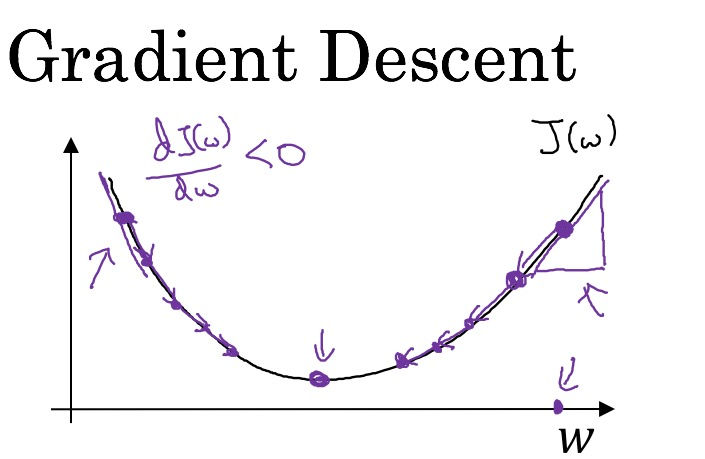
\includegraphics[width=25em]{figures/1-gradient-descent}
    \caption{Gradient descent. (Ignore $b$ here)}
\end{figure}

\begin{algorithm}[ht]
\Repeat{iteration = MaxIteration}{
        $\displaystyle{w := w - \alpha \frac{\partial J(w)}{\partial w}}$ \\
        $\displaystyle{b := b - \alpha \frac{\partial J(w)}{\partial b}}$
}
\end{algorithm}

Note: We often use ``d$w$'' to denote $\displaystyle{\frac{\partial J(w)}{\partial w}}$, use
``d$b$'' to denote $\displaystyle{\frac{\partial J(w)}{\partial b}}$. In other words, we use
``d$var$'' to denote $\displaystyle\frac{\text{d}FinalOutputVar}{\text{d}var}$ or
$\displaystyle\frac{\partial FinalOutputVar}{\partial var}$.

\paragraph{Gradient on single example:}
\begin{IEEEeqnarray*}{rCl}
    z = w^T x + b
\end{IEEEeqnarray*}

\begin{IEEEeqnarray*}{rCl}
    \hat{y} = a = \sigma(z) = \frac{1}{1 + e^{-z}}
\end{IEEEeqnarray*}

\begin{IEEEeqnarray*}{rCl}
    \Cal{L}(a, y) = -(y\log(a) + (1-y)\log(1-a))
\end{IEEEeqnarray*}

\begin{figure}[ht]
    \centering
    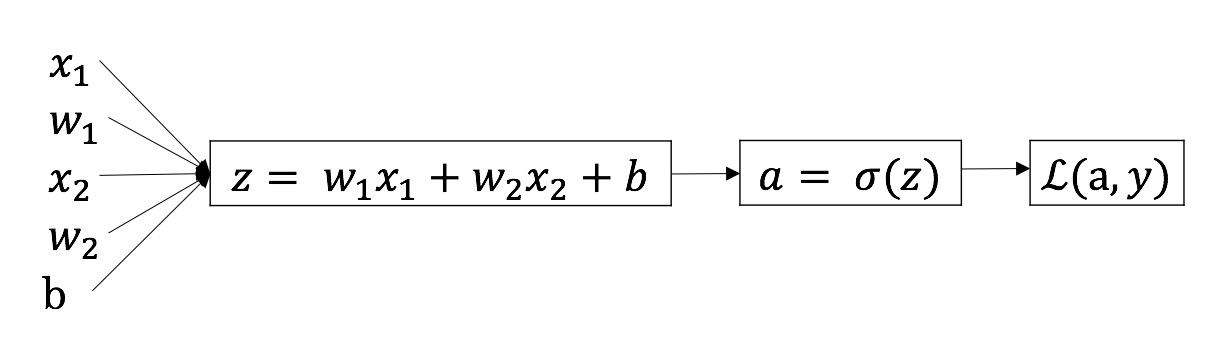
\includegraphics[width=35em]{figures/1-lr-gradient-descent}
    \caption{The computation graph of logistic regression gradient descent}
    \label{fig:1-lr-gradient-descent}
\end{figure}

According to the computation graph~\ref{fig:1-lr-gradient-descent}, go backwards to compute the
derivatives:
\begin{IEEEeqnarray*}{rCl}
    \text{d}a = \frac{\text{d}\Cal{L}(a, y)}{\text{d}a} = -\frac{y}{a} + \frac{1-y}{1-a}
\end{IEEEeqnarray*}

\begin{IEEEeqnarray*}{rCl}
    \text{d}z = \frac{\text{d}\Cal{L}(a, y)}{\text{d}z} = \frac{\text{d}\Cal{L}}{\text{d}a} \cdot
    \frac{\text{d}a}{\text{d}z} = (-\frac{y}{a} + \frac{1-y}{1-a}) \cdot a(1-a) = a - y
\end{IEEEeqnarray*}

\begin{IEEEeqnarray*}{rCl}
    \text{d}w_1 = \frac{\partial \Cal{L}}{\partial w_1} = x_1 \text{d}z = x_1 (a-y)
\end{IEEEeqnarray*}

\begin{IEEEeqnarray*}{rCl}
    \text{d}w_2 = \frac{\partial \Cal{L}}{\partial w_2} = x_2 \text{d}z = x_2 (a-y)
\end{IEEEeqnarray*}

\begin{IEEEeqnarray*}{rCl}
    \text{d}b = \frac{\partial \Cal{L}}{\partial b} = \text{d}z = a - y
\end{IEEEeqnarray*}

\paragraph{Gradient on m examples:}
\begin{IEEEeqnarray*}{rCl}
    J(w, b) = \frac{1}{m} \sum_{i=1}^m \Cal{L}(a^{(i)}, y^{(i)})
\end{IEEEeqnarray*}

\begin{IEEEeqnarray*}{rCl}
    a^{(i)} = \hat{y^{(i)}} = \sigma(z^{(i)}) = \sigma(w^T x^{(i)} + b)
\end{IEEEeqnarray*}

\begin{IEEEeqnarray*}{rCl}
    \frac{\partial J(w, b)}{\partial w_1} = \frac{1}{m} \sum_{i=1}^m
    \frac{\partial \Cal{L}(a^{(i)}, y^{(i)})}{\partial w_1} = \frac{1}{m} \sum_{i=1}^m \text{d}w_1^{(i)}
\end{IEEEeqnarray*}

The following is the algorithm of Logistic Regression Gradient Descent on m examples. It uses two
for-loops, so it's less efficient than use vertorization.
\begin{algorithm}[ht]
    \tcc{Initialization}
    $J = 0;$ \\
    \For{$j = 1$ \KwTo $n$}{
        $\text{d}w_j = 0$ \\
    }
    $\text{d}b = 0;$

    \tcc{Compute cost and derivatives}
    \For{$i = 0$ \KwTo $m$}{
        $z^{(i)} = w^T x^{(i)} + b;$ \\
        $a^{(i)} = \sigma(z^{(i)});$ \\
        $J = J - [y^{(i)} \log a^{(i)} + (1-y^{(i)})\log (1-a^{(i)})];$ \\
        $\text{d}z^{(i)} = a^{(i)} - y^{(i)};$ \\
        \For{$j = 1$ \KwTo $n$}{
            $\text{d}w_j = \text{d}w_j + x_j^{(i)} \text{d}z^{(i)};$ \\
        }
        $\text{d}b = \text{d}b + \text{d}z^{(i)}$
    }

    \tcc{Get the average}
    $J = J / m;$ \\
    \For{$j = 1$ \KwTo $n$}{
        $\text{d}w_j = \text{d}w_j / m$
    }
    $\text{d}b = \text{d}b / m;$

    \tcc{Gradient descent}
    \For{$j = 1$ \KwTo $n$}{
        $\text{d}w_j = \text{d}w_j - \alpha \text{d}w_j$
    }
    $b = b - \alpha \text{d}b$
\end{algorithm}











\end{document}
